\documentclass[10pt]{article}
\usepackage[margin=1in, paperwidth=8.5in, paperheight=11in]{geometry}
\usepackage{ifpdf, amsmath, amssymb, comment, color, graphicx, stmaryrd, setspace, enumitem, fancyhdr, wrapfig, textcomp, mathptmx, siunitx, multicol}
\usepackage{hyperref}
\hypersetup{
    colorlinks=true,
    urlcolor=blue,
}

\usepackage{tikz}
\usetikzlibrary{trees}

\setlength{\headheight}{14.5pt}
\newcommand{\del}{\nabla}
\newcommand{\Q}{\mathbb{Q}}
\newcommand{\R}{\mathbb{R}}
\newcommand{\Z}{\mathbb{Z}}
\newcommand{\vu}{\mathbf{u}}
\newcommand{\vv}{\mathbf{v}}
\newcommand{\vw}{\mathbf{w}}
\newcommand{\vi}{\mathbf{i}}
\newcommand{\vj}{\mathbf{j}}
\newcommand{\vk}{\mathbf{k}}
\newcommand{\vn}{\mathbf{n}}
\newcommand{\vr}{\mathbf{r}}
\newcommand{\vs}{\mathbf{s}}
\newcommand{\va}{\mathbf{a}}
\newcommand{\vF}{\mathbf{F}}
\newcommand{\vL}{\mathbf{L}}
\newcommand{\vT}{\mathbf{T}}
\newcommand{\vN}{\mathbf{N}}
\newcommand{\vB}{\mathbf{B}}
\newcommand{\comp}{\operatorname{comp}}
\newcommand{\proj}{\operatorname{proj}}
\newcommand{\orth}{\operatorname{orth}}
\newcommand\dotp[1][.5]{\,\mathbin{\vcenter{\hbox{\scalebox{#1}{$\bullet$}}}}\,}


\newenvironment{red}{\color{red}}{\ignorespacesafterend}
\newcommand{\blue}[1]{\textcolor{blue}{#1}}
\newcommand{\green}[1]{\textcolor{green}{#1}}
\renewcommand{\section}[1]{\begin{center} \textbf{#1} \\\end{center}}
%
\hyphenpenalty=5000
\setlength{\parindent}{0in}
%\oddsidemargin=-.25in
\allowdisplaybreaks
\pagestyle{fancy}
\renewcommand{\headrulewidth}{0pt}
\lhead{MATH 203}
\rhead{Fall 2024}
%\lfoot{}
%\cfoot{}

\begin{document}
%


%\onehalfspacing
\allowdisplaybreaks
%##################################################################
\section{PS\#9 - Constrained optimization - \red{Answer key} }


\begin{enumerate}[leftmargin=0pt]
    
    \item In CalcPlot3D, graph the function $f(x,y) = 2- x^2 - y^2$. Based on the graph, does this function have any critical points? If so, where, and what kind?
    \begin{center}
        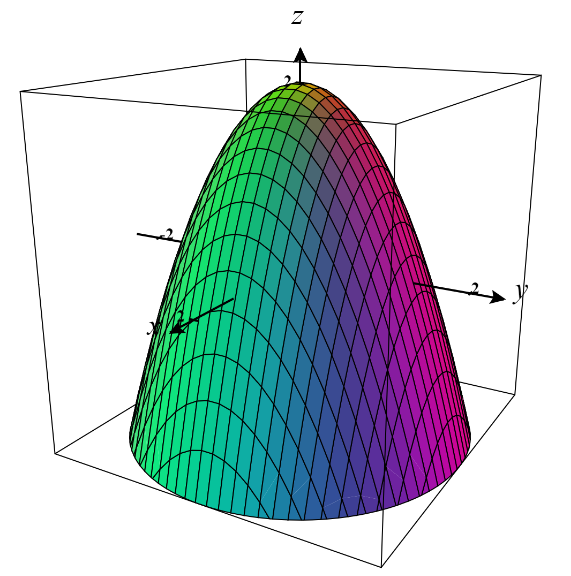
\includegraphics[width=0.5\textwidth]{../images/constrained-optimization/plot1.png}
    \end{center}
    
    \begin{red}
    Looks like there's one maximum at $(0,0)$.
    \end{red}
    \item Confirm your answers to part 1: Use the methods in section 10.7 to locate and classify any critical points of this function.
    
    \begin{red}
    Ok, so we need to compute $\del f$ and find where it equals $\mathbf{0}$. $\del f = \langle -2x, -2y\rangle = \langle0, 0\rangle$ implies that $x=0$ and $y=0$, so indeed $(0, 0)$ is the only critical point.
    
    Now let's compute the discriminant $D$. I'll need all the second derivatives first:
    \[\begin{array}{cc}
        f_{xx} = -2 & f_{yx} = 0 \\
        f_{xy} = 0 & f_{yy} = -2
    \end{array}
    \]
    Now $D = f_{xx} f_{yy} - f_{xy}^2 = (-2)(-2) - (0)^2 = 4 > 0$. So I know I'm at either a max or a min. To tell which, I just note that $f_{xx} < 0$ (and so is $f_{yy}$), so the traces are concave down, which means we're for sure at a maximum. Yay, that confirms my thinking from part 1.
    \end{red}
    
    \pagebreak
    
    \item Now consider the ellipse $1/4 (x-1)^2 + y^2 = 1$. I'll tell you for free that you can parameterize this as follows:
    \begin{align*}
        x(t) &= 2 \cos(t) + 1\\
        y(t) &= \sin(t) \\
        z(t) &= 0 \\
        0 &\leq t \leq 2\pi
    \end{align*}
    Plot this as a two-dimensional space curve on the same axes in CalcPlot3D.
    \begin{center}
        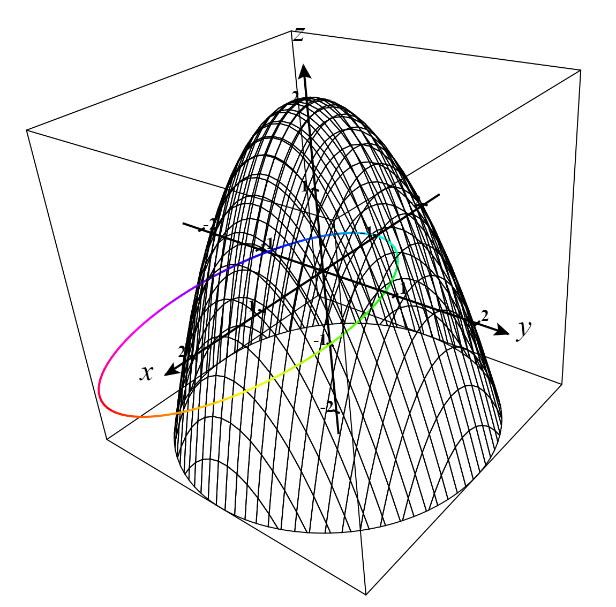
\includegraphics[width=0.5\textwidth]{../images/constrained-optimization/plot3.png}
    \end{center}
    \begin{red}
    (I turned off the faces and just left the wireframe in so that you can see the curve through the function.)
    \end{red}
    
    \item Now we'd like to ``lift'' this path up onto the surface $f(x, y)$. This is easy enough: replace $z(t) = 0$ by what you would get if you plugged $x(t)$ and $y(t)$ into the equation for $f(x, y)$. Draw this in CalcPlot3D. \\
    Based on your examination of the resulting plot, where would you estimate are the highest and lowest points on $f(x, y)$ \textbf{along this curve}? (Eyeball it.)
    
    \begin{center}
        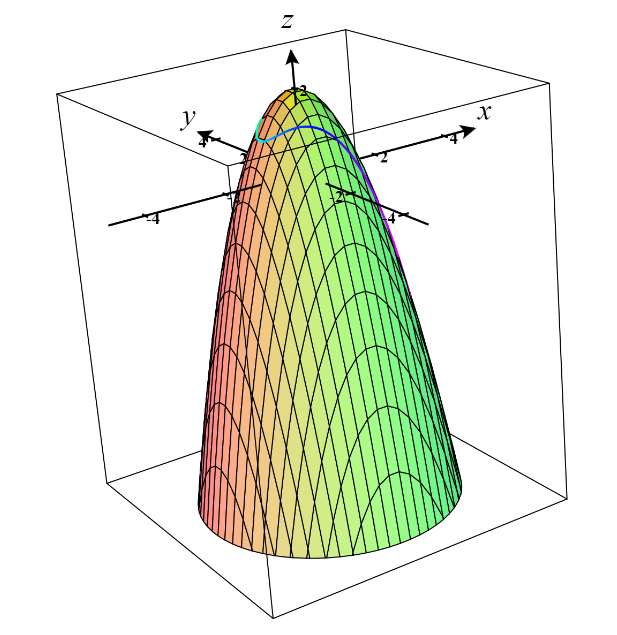
\includegraphics[width=0.3\textwidth]{../images/constrained-optimization/plot4-3.png}
        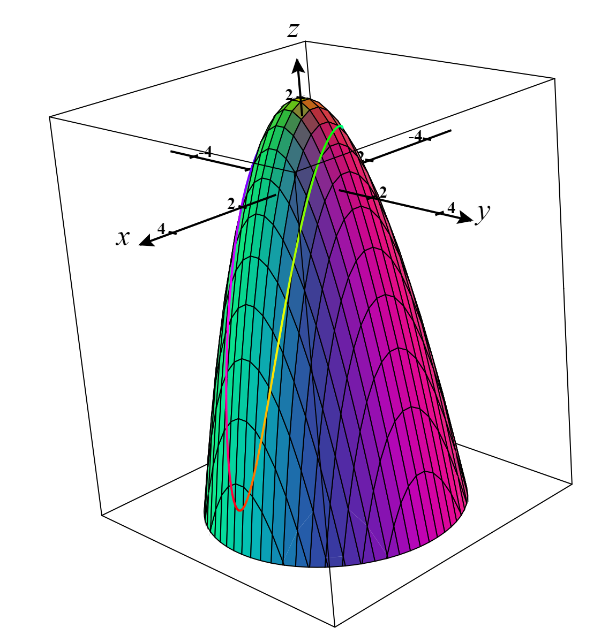
\includegraphics[width=0.3\textwidth]{../images/constrained-optimization/plot4-1.png}
        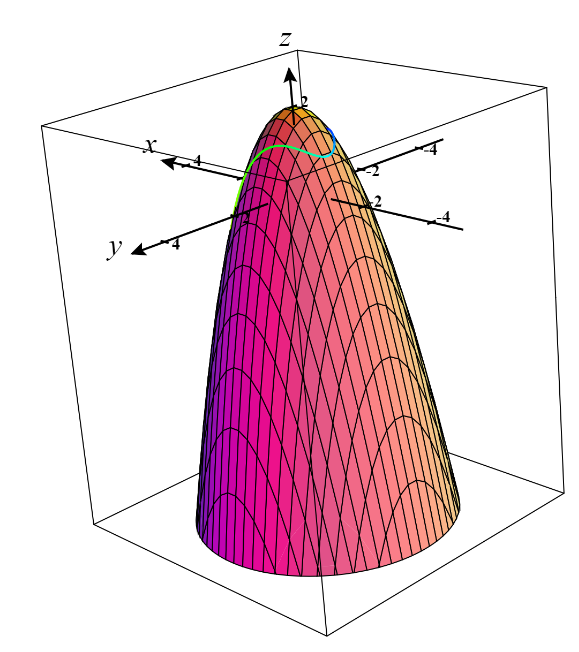
\includegraphics[width=0.3\textwidth]{../images/constrained-optimization/plot4-2.png}
    \end{center}
    
    \begin{red}
    So based on these pictures (which I've obtained by rotating the plot around the $z$-axis), looks like I've got a way low point at maybe $x=3$ and $y=0$; a medium low point at maybe $x=-1$ and $y=0$; and then a pair of high points at maybe $x=-1/2$ and maybe $y=\pm 1$.
    \end{red}
    
    \item Confirm your answers to part 4: Use the methods in section 10.8 to locate the extrema of $f(x, y)$ subject to the constraint that $1/4 (x-1)^2 + y^2 = 1$.
    
    \begin{red}
    Setting up the Lagrange multipliers thing, we need to calculate $\del f = \langle -2x, -2y \rangle$ and $\del g = \langle 1/2 (x-1), 2y \rangle$. Therefore we get the following system of equations:
    \begin{align*}
        -2x &= \lambda \cdot 1/2 (x-1) \\
        -2y &= \lambda \cdot 2y \\
        1   &= 1/4 (x-1)^2 + y^2
    \end{align*}
    You can certainly solve this system of equations by hand, and that's what I made \href{https://youtu.be/7ksSX-Z7yKo}{this video} about. But, let's make computers do our dirty work for us.
    \end{red}
    \begin{center}
        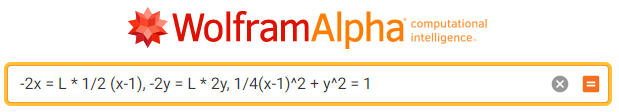
\includegraphics[width=0.7\textwidth]{../images/constrained-optimization/wa-input.png}
        
        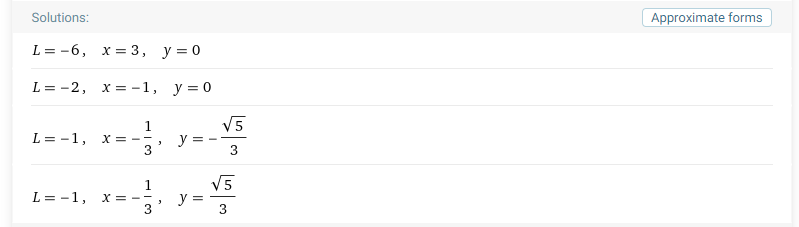
\includegraphics[width=0.7\textwidth]{../images/constrained-optimization/wa-output.png}
    \end{center}
    \begin{red}
    Hey, that actually lines up pretty well with our guesses.
    \end{red}
    
    \item Put it all together: If we're just looking inside this ellipse or on its boundary, what is the \textbf{absolute maximum} of $f(x, y)$, and where does it occur? What is the \textbf{absolute minimum} of $f(x, y)$, and where does it occur?
    
    \begin{red}
    So now we know the locations of five interesting points on our function. In order to find out which one produces the very biggest and which one produces the very smallest function values, we just need to feed each of them into the function and compare the outputs.
    \begin{align*}
        f(0, 0) &= 2 \\
        f(3, 0) &= -7 \\
        f(-1, 0) &= 1 \\
        f(-1/3, \sqrt{5}/3) &= 1.2723 \\
        f(-1/3, -\sqrt{5}/3) &= 1.2723 
    \end{align*}
    The very highest of this constellation of values is 2, so $(0,0)$ is the location of the absolute maximum. The very lowest of this constellation of values is $-7$, so $(3, 0)$ is the location of the absolute minimum.
    \end{red}
        
\end{enumerate}

\end{document}